\documentclass{standalone}
\usepackage{tikz,xcolor,amsmath}
\usetikzlibrary{shapes.geometric}
\begin{document}
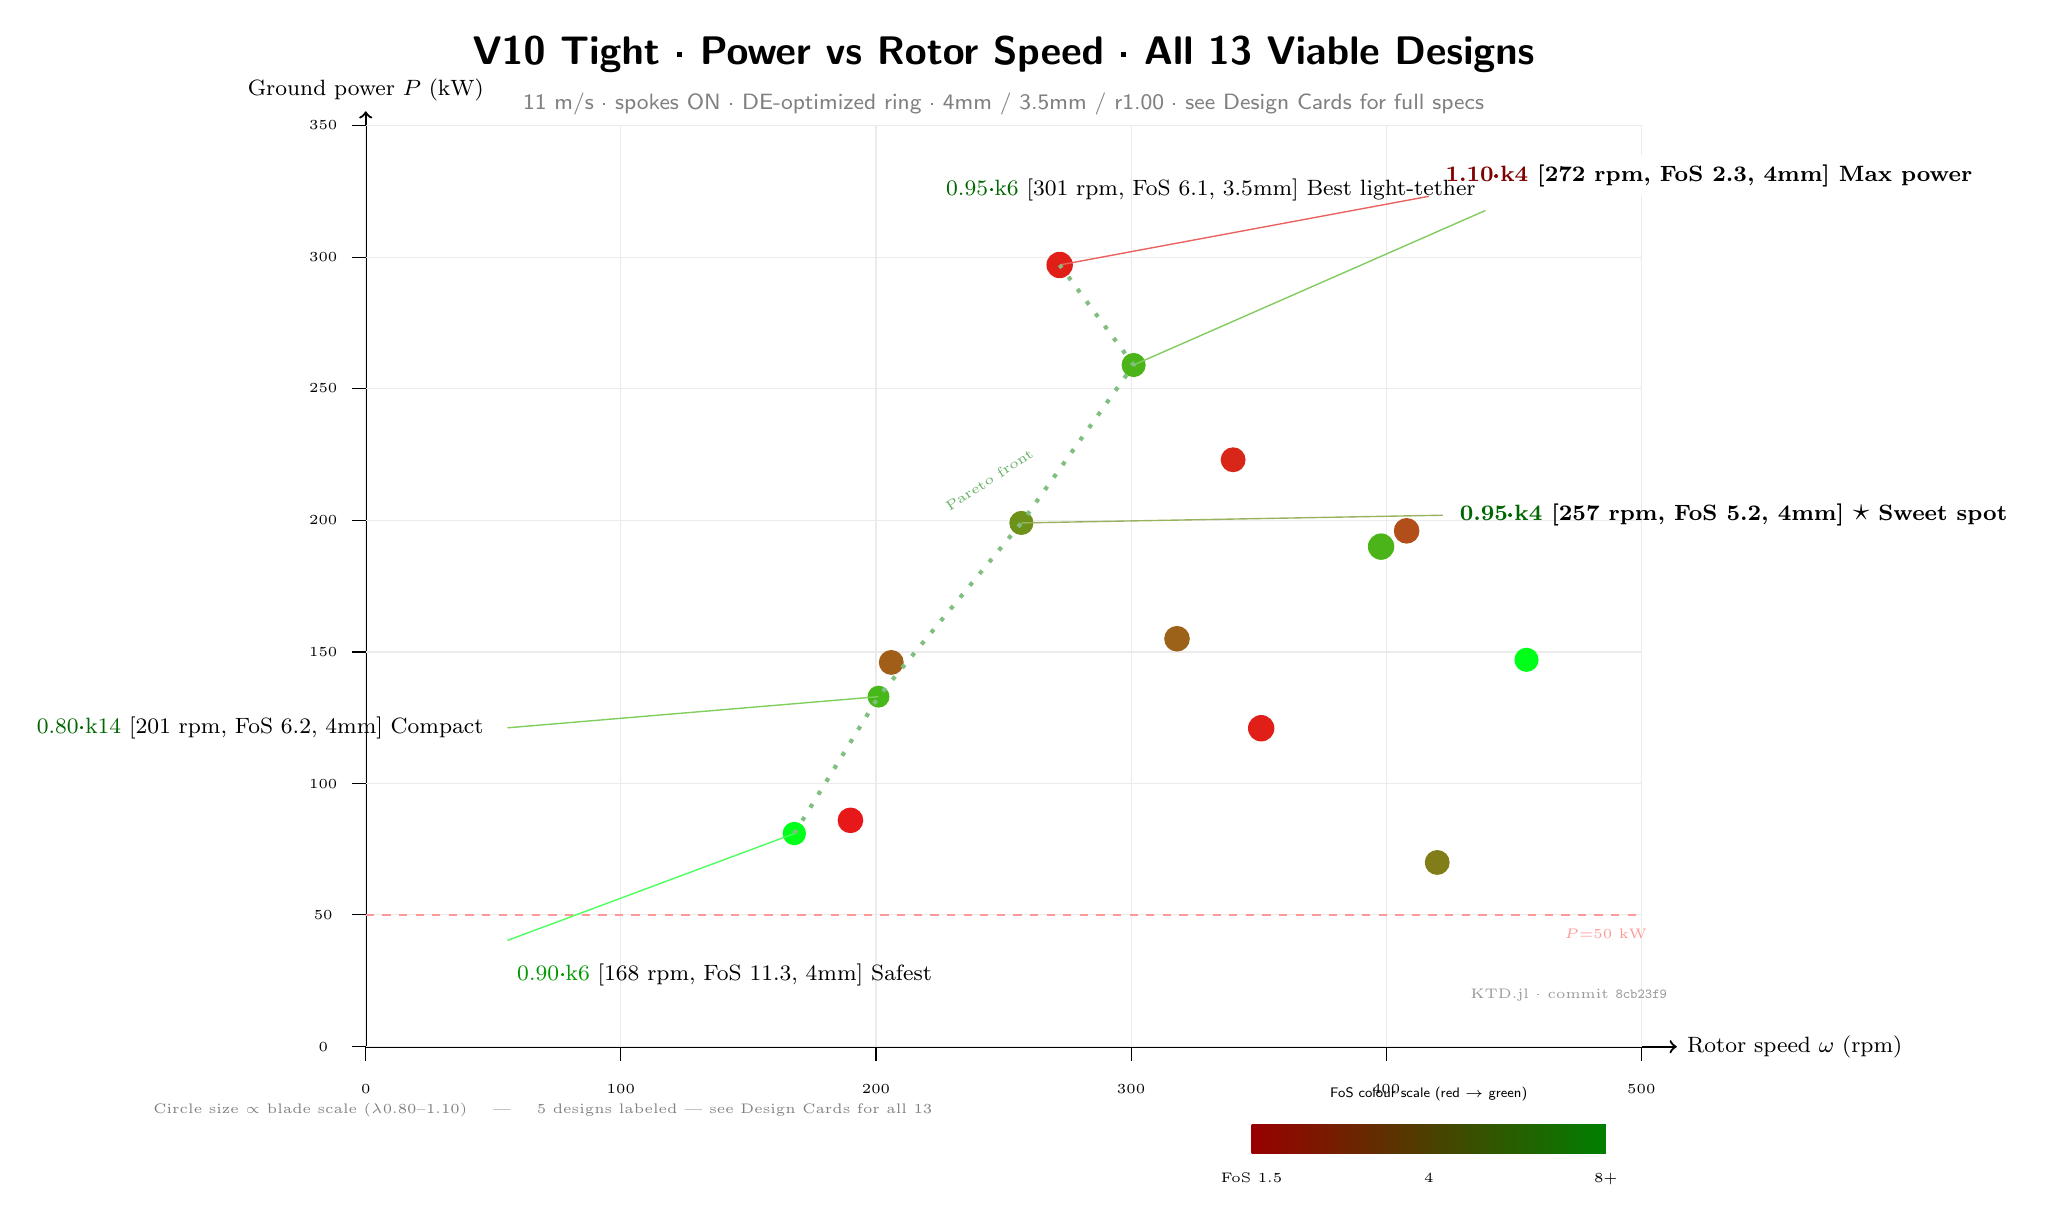
\begin{tikzpicture}[scale=0.90]

% ── Title ──
\node[font=\Large\sffamily\bfseries] at (11.0, 16.0) {V10 Tight · Power vs Rotor Speed · All 13 Viable Designs};
\node[font=\footnotesize\sffamily, black!50] at (11.0, 15.3) {11 m/s · spokes ON · DE-optimized ring · 4mm / 3.5mm / r1.00 · see Design Cards for full specs};

% ── Axes: x=2.0+ω*18/500, y=2.0+P*13/350 ──
\draw[->, thick] (2.0, 2.0) -- (20.5, 2.0) node[right, font=\footnotesize] {Rotor speed $\omega$ (rpm)};
\draw[->, thick] (2.0, 2.0) -- (2.0, 15.2) node[above, font=\footnotesize] {Ground power $P$ (kW)};

% Grid
\foreach \w/\x in {0/2.0, 100/5.6, 200/9.2, 300/12.8, 400/16.4, 500/20.0} {
  \draw[black!8] (\x, 2.0) -- (\x, 15.0);
  \draw (\x, 1.8) -- (\x, 2.0);
  \node[font=\tiny] at (\x, 1.4) {\w};
}
\foreach \p/\y in {0/2.0, 50/3.86, 100/5.71, 150/7.57, 200/9.43, 250/11.29, 300/13.14, 350/15.0} {
  \draw[black!8] (2.0, \y) -- (20.0, \y);
  \draw (1.8, \y) -- (2.0, \y);
  \node[font=\tiny] at (1.4, \y) {\p};
}

% Gate
\draw[dashed, red!40, line width=0.5pt] (2.0, 3.86) -- (20.0, 3.86);
\node[font=\tiny, red!40] at (19.5, 3.6) {$P{=}50$ kW};

% ── Helpers ──
\def\px#1{2.0 + #1/500*18}
\def\py#1{2.0 + #1/350*13}
\def\siz#1{2.0 + #1*3.0}

% ── FoS → continuous red→amber→green color function ──
% FoS 1.5 = red, FoS 4 = amber, FoS 8+ = green
\def\foscol#1{%
  \pgfmathsetmacro{\f}{#1}%
  \pgfmathsetmacro{\rf}{max(0, min(1, (8.0-\f)/6.5))}% red: 1 at FoS=1.5, 0 at FoS=8
  \pgfmathsetmacro{\gf}{max(0, min(1, (\f-1.5)/6.5))}% green: 0 at FoS=1.5, 1 at FoS=8
  \pgfmathsetmacro{\bf}{0.1}%
  \definecolor{ptcol}{rgb}{\rf,\gf,\bf}%
}

% ══════════════════════════════════════════════════
% ALL 13 DATA POINTS — sorted by FoS
% ══════════════════════════════════════════════════

% 1. 0.90·k6    (81 kW, 168 rpm, FoS 11.3)
\foscol{11.3}\fill[ptcol] (\px{168}, \py{81}) circle (\siz{0.90} pt);

% 2. 0.95·k2ʳ   (147, 455, 8.6)
\foscol{8.6}\fill[ptcol] (\px{455}, \py{147}) circle (\siz{0.95} pt);

% 3. 0.80·k14   (133, 201, 6.2)
\foscol{6.2}\fill[ptcol] (\px{201}, \py{133}) circle (\siz{0.80} pt);

% 4. 0.95·k6³·⁵ (259, 301, 6.1)
\foscol{6.1}\fill[ptcol] (\px{301}, \py{259}) circle (\siz{0.95} pt);

% 5. 1.10·k2ʳ   (190, 398, 6.1)
\foscol{6.1}\fill[ptcol] (\px{398}, \py{190}) circle (\siz{1.10} pt);

% 6. 0.95·k4    (199, 257, 5.2) — SWEET SPOT
\foscol{5.2}\fill[ptcol] (\px{257}, \py{199}) circle (\siz{0.95} pt);

% 7. 1.00·k2ʳ   (70, ~420, 4.7)
\foscol{4.7}\fill[ptcol] (\px{420}, \py{70}) circle (\siz{1.00} pt);

% 8. 1.05·k2³·⁵ (155, 318, 4.0)
\foscol{4.0}\fill[ptcol] (\px{318}, \py{155}) circle (\siz{1.05} pt);

% 9. 1.00·k4    (146, 206, 3.9)
\foscol{3.9}\fill[ptcol] (\px{206}, \py{146}) circle (\siz{1.00} pt);

% 10. 1.05·k2ʳ  (196, 408, 3.5)
\foscol{3.5}\fill[ptcol] (\px{408}, \py{196}) circle (\siz{1.05} pt);

% 11. 1.00·k2³·⁵ (223, ~340, 2.5)
\foscol{2.5}\fill[ptcol] (\px{340}, \py{223}) circle (\siz{1.00} pt);

% 12. 1.10·k4   (297, 272, 2.3) — MAX POWER
\foscol{2.3}\fill[ptcol] (\px{272}, \py{297}) circle (\siz{1.10} pt);

% 13. 1.10·k2³·⁵(121, 351, 2.3)
\foscol{2.3}\fill[ptcol] (\px{351}, \py{121}) circle (\siz{1.10} pt);

% 14. 1.05·k4   (86, 190, 2.1)
\foscol{2.1}\fill[ptcol] (\px{190}, \py{86}) circle (\siz{1.05} pt);

% ══════════════════════════════════════════════════
% LABELS — short bracketed format: [ω, FoS, variant]
% Only 5 key designs labeled
% ══════════════════════════════════════════════════

% Sweet spot — 0.95·k4 [257, 5.2, 4mm]
\foscol{5.2}
\draw[ptcol!70, line width=0.5pt] (\px{257}, \py{199}) -- (17.2, 9.5);
\node[font=\footnotesize\bfseries, anchor=west] at (17.3, 9.5) {\textcolor{green!40!black}{0.95·k4} [257 rpm, FoS 5.2, 4mm] {\large$\star$} Sweet spot};

% Max power — 1.10·k4 [272, 2.3, 4mm]  (leader line to RIGHT, avoiding title)
\foscol{2.3}
\draw[ptcol!70, line width=0.5pt] (\px{272}, \py{297}) -- (17.0, 14.0);
\node[font=\footnotesize\bfseries, anchor=south west, fill=white, fill opacity=0.9, text opacity=1] at (17.1, 14.0) {\textcolor{red!50!black}{1.10·k4} [272 rpm, FoS 2.3, 4mm] Max power};

% Safest — 0.90·k6 [168, 11.3, 4mm]
\foscol{11.3}
\draw[ptcol!70, line width=0.5pt] (\px{168}, \py{81}) -- (4.0, 3.5);
\node[font=\footnotesize, anchor=north west] at (4.0, 3.3) {\textcolor{green!60!black}{0.90·k6} [168 rpm, FoS 11.3, 4mm] Safest};

% Best light-tether — 0.95·k6³·⁵ [301, 6.1, 3.5mm]
\foscol{6.1}
\draw[ptcol!70, line width=0.5pt] (\px{301}, \py{259}) -- (17.8, 13.8);
\node[font=\footnotesize, anchor=south east] at (17.8, 13.8) {\textcolor{green!40!black}{0.95·k6} [301 rpm, FoS 6.1, 3.5mm] Best light-tether};

% Compact — 0.80·k14 [201, 6.2, 4mm]
\foscol{6.2}
\draw[ptcol!70, line width=0.5pt] (\px{201}, \py{133}) -- (4.0, 6.5);
\node[font=\footnotesize, anchor=east] at (3.8, 6.5) {\textcolor{green!40!black}{0.80·k14} [201 rpm, FoS 6.2, 4mm] Compact};

% ══════════════════════════════════════════════════
% PARETO FRONTIER
% ══════════════════════════════════════════════════
\draw[green!50!black!50, line width=1.5pt, loosely dotted] 
  (\px{168}, \py{81})  -- (\px{201}, \py{133}) -- (\px{257}, \py{199}) 
  -- (\px{301}, \py{259}) -- (\px{272}, \py{297});
\node[green!50!black!60, font=\tiny, rotate=33] at (10.8, 10.0) {Pareto front};

% ══════════════════════════════════════════════════
% FoS COLOR BAR (continuous spectrum)
% ══════════════════════════════════════════════════
\shade[left color=red!60!black, right color=green!50!black] (14.5, 0.5) rectangle (19.5, 0.9);
\node[font=\tiny, below] at (14.5, 0.35) {FoS 1.5};
\node[font=\tiny, below] at (17.0, 0.35) {4};
\node[font=\tiny, below] at (19.5, 0.35) {8+};
\node[font=\tiny\sffamily, above] at (17.0, 1.1) {FoS colour scale (red $\rightarrow$ green)};

% Size legend
\node[font=\tiny, black!50] at (4.5, 1.1) {Circle size $\propto$ blade scale ($\lambda$0.80--1.10) \quad | \quad 5 designs labeled --- see Design Cards for all 13};

% ── Data box ──
\node[font=\tiny, black!40, anchor=south east] at (20.5, 2.5) {KTD.jl · commit \texttt{8cb23f9}};

\end{tikzpicture}
\end{document}
